\documentclass[11pt]{beamer}
\usetheme{Boadilla}
\usepackage[utf8]{inputenc}
\usepackage{amsmath}
\usepackage{amsfonts}
\usepackage{amssymb}
\usepackage{tabularx}
\graphicspath{{fig/}}
\author[WK, JSM, JEB, and SAB]{Weiyao Ke, J Scott Moreland, Jonah E Bernhard,
		and Steffen A Bass}
\title[3D Initial Condition]{Constraining 3D Hydrodynamic Initial Condition for Relativistic
		Heavy-ion Collisions from Multiplicity Observables
		of pA and AA @LHC }
%\setbeamercovered{transparent}
%\setbeamertemplate{navigation symbols}{}
%\logo{}
%\institute{}
%\date{}
%\subject{}
\begin{document}

\begin{frame}
\titlepage
\end{frame}

\begin{frame}
\tableofcontents
\end{frame}

\section{Introduction: initial condition for 3+1D simulation}
\begin{frame}{A more complete and detailed space-time evolution}
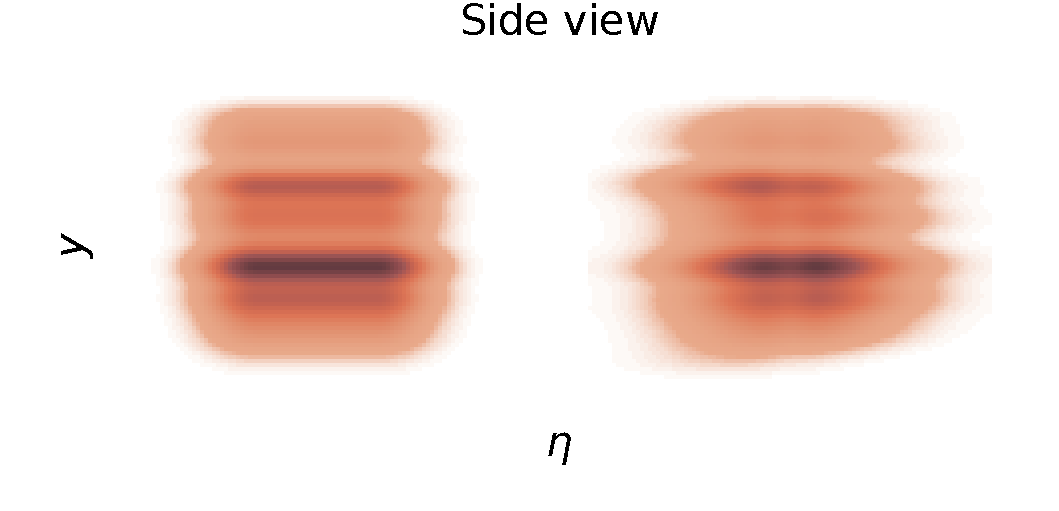
\includegraphics[width=0.6\textwidth]{nuclei_demo.pdf}
\end{frame}

\begin{frame}{Importance of asymmetry and fluctuation}

\end{frame}

\section{Parametric longitudinal information}
\begin{frame}{A cumulant generating approach}
\begin{itemize}
\item Extending a midrapidity initial condition to finite rapidity.
\begin{eqnarray}\nonumber 
\frac{dS}{\tau dx_\perp^2d \eta} &=& \frac{1}{\tau}s(\vec{x}_\perp, \eta) =  \frac{\tau_0}{\tau} {\color{red} s_0(\vec{x}_\perp)} {\color{blue}f(y, x_\perp)} \frac{dy}{d\eta}
\end{eqnarray} 
\item {\color{red} $s_0(\vec{x}_\perp)$}: a boost-invariant model. {\color{blue} $f(y, x_\perp)$}: the functional form for $x_\perp$-local rapidity profile, granted with three degrees of freedom: \\
mean ($\mu$), std ($\sigma$), skewness ($\gamma$).
\begin{eqnarray}\nonumber 
f(y) &=& \mathcal{F}^{-1}\{\tilde{f}(k)\}	\\ \nonumber 
\tilde{f}(k) &\propto & \exp\left\{ik\mu(x_\perp) -\frac{1}{2}[\sigma(x_\perp) k]^2 - \frac{i}{6}\gamma(x_\perp)[\sigma(x_\perp) k]^3 + ...\right\}
\end{eqnarray}
\item Parametrization: $f(y)$ asymmetry $\leftarrow$ local $T_A$, $T_B$ asymmetry.
\end{itemize}
\begin{center}
\begin{tabularx}{0.95\textwidth}{p{2.5cm}p{1.cm}p{8cm}}
\hline
mean & std & absolute or relative-skewness \\
\hline
\noalign{\smallskip}
$\mu_0 \log\frac{T_A(x_\perp)}{T_B(x_\perp)}$ & $\sigma_0$ & $\gamma_0(T_A(x_\perp)-T_B(x_\perp))$ or $\gamma_0\frac{T_A(x_\perp)-T_B(x_\perp)}{T_A(x_\perp)+T_B(x_\perp)}$ \\
\noalign{\smallskip}
\hline
\end{tabularx}
\end{center}
\end{frame}

\begin{frame}{Realizations}
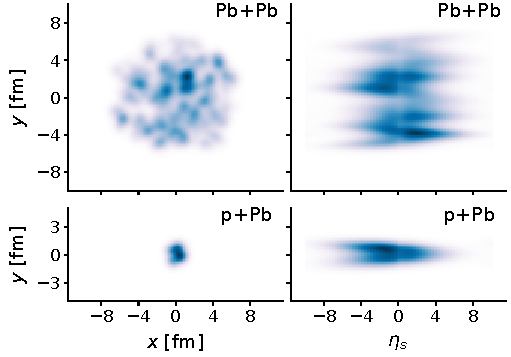
\includegraphics[width=0.5\textwidth]{trento3d_example.pdf}
\end{frame}

\section{Model to data comparison}
\begin{frame}{Bayesian model-to-data comparison}

\end{frame}
\begin{frame}{Multiplicity observable as calibration data.}

\end{frame}

\section{Constraint initial condition and predictions}
\begin{frame}{Posterior observables}
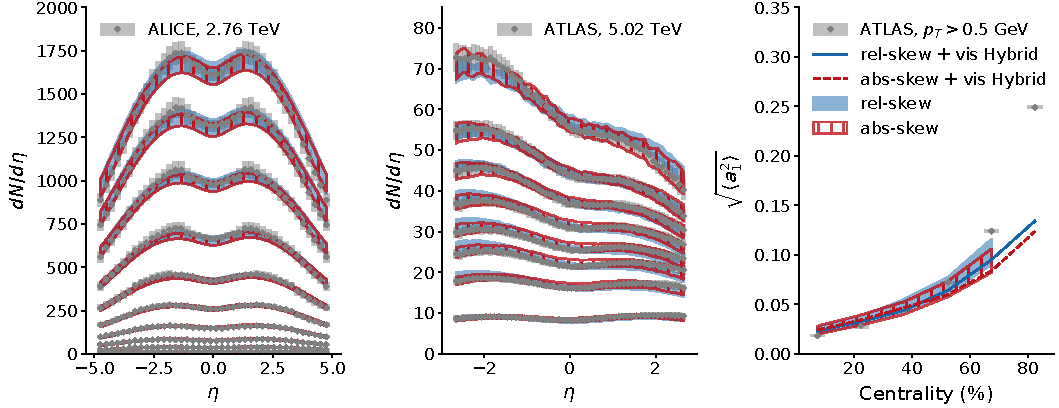
\includegraphics[width=\textwidth]{post_obs.pdf}
\end{frame}

\begin{frame}{The constraint initial condition}
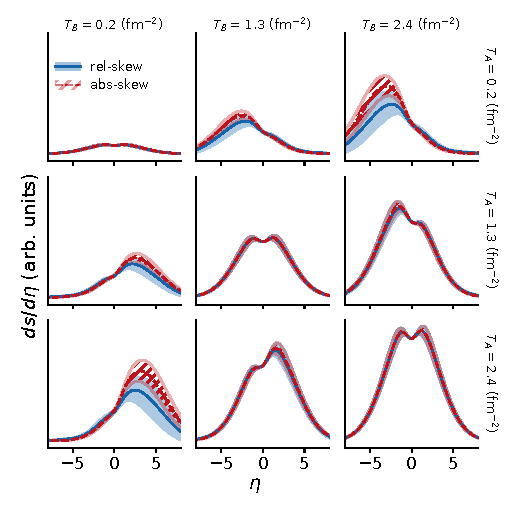
\includegraphics[width=0.6\textwidth]{post_dsdy.pdf}
\end{frame}

\begin{frame}{Prediction on azimuthal observables}
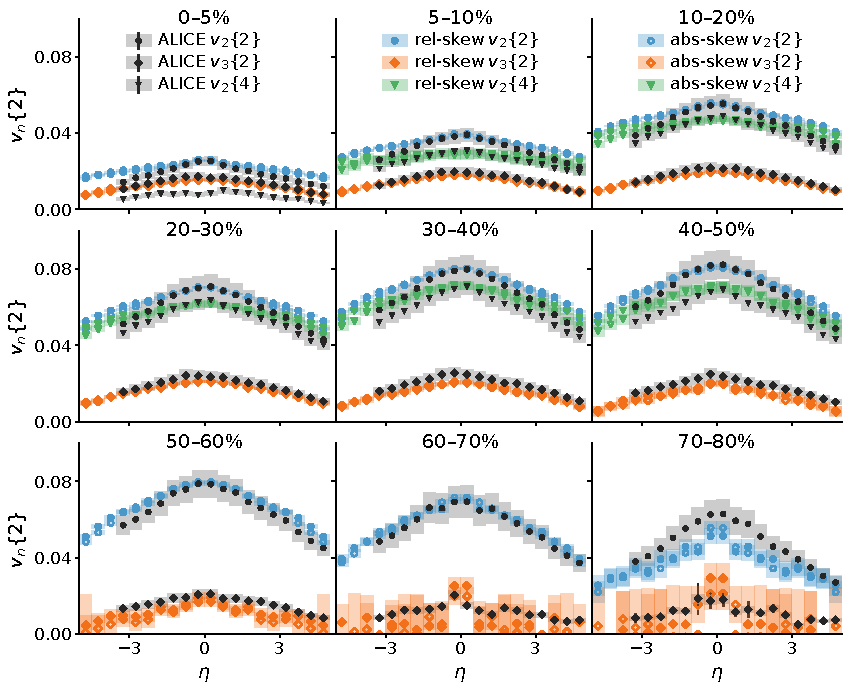
\includegraphics[width=0.7\textwidth]{vn_eta.pdf}
\end{frame}

\begin{frame}{Event plane decorrelation}
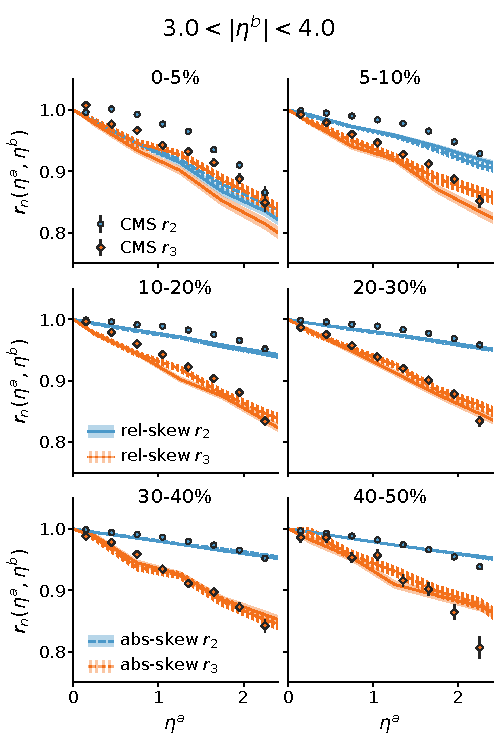
\includegraphics[width=0.4\textwidth]{evt_pln_decorr_near.pdf}
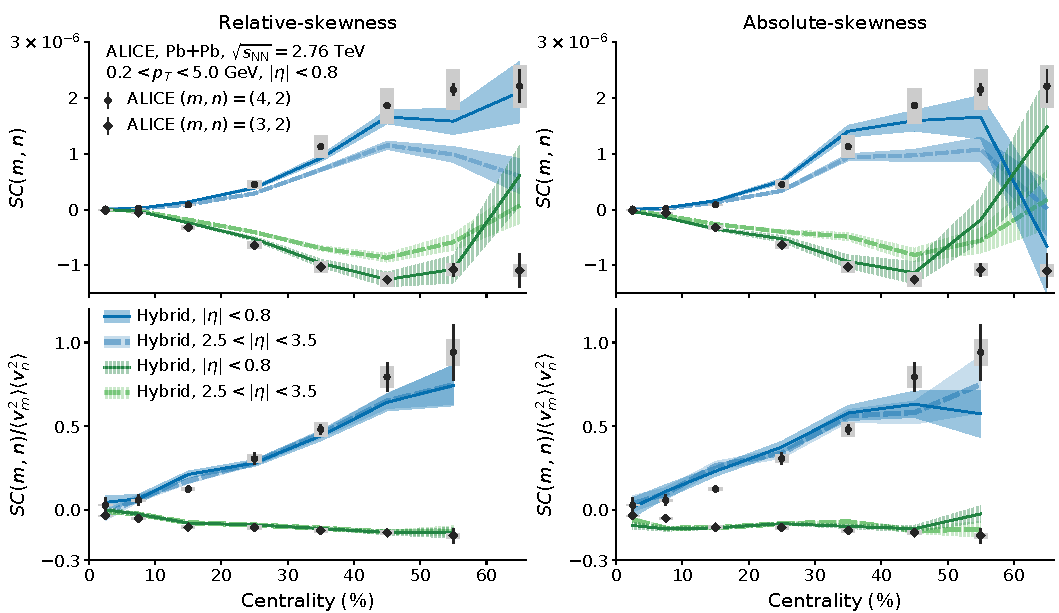
\includegraphics[width=0.6\textwidth]{smn.pdf}
\end{frame}

\begin{frame}{Summary}
\end{frame}

\end{document}
